\section{MLP training}\label{sec:activitytraining}

Script \texttt{mlptrain\_act.m} is the adaptation of the script used in
\secref{sec:mlptraining} for the activity recognition network. It performs the
training used the architecture and hyperparameters selected in
\secref{subsec:activitybayesopt} and the training algorithm selected in
\secref{subsec:activityhyperopt} \idest{\code{trainscg}}.

\vfigref{fig:activityconfusion} shows the confusion matrices for the network.
The Receiver Operating Characteristic (ROC) curves are shown in
\vfigref{fig:activityroc}. The network is able to achieve very good results
with only \(2.3\%\) of samples misclassified for the test set and \(1.7\%\) of
samples misclassified for the entire dataset. As shown in the confusion
matrices, the network sometimes misclassifies samples belonging to the ``sit''
class, while it never fails for the other 2 classes.

\begin{figure}[htbp]
	\centering
	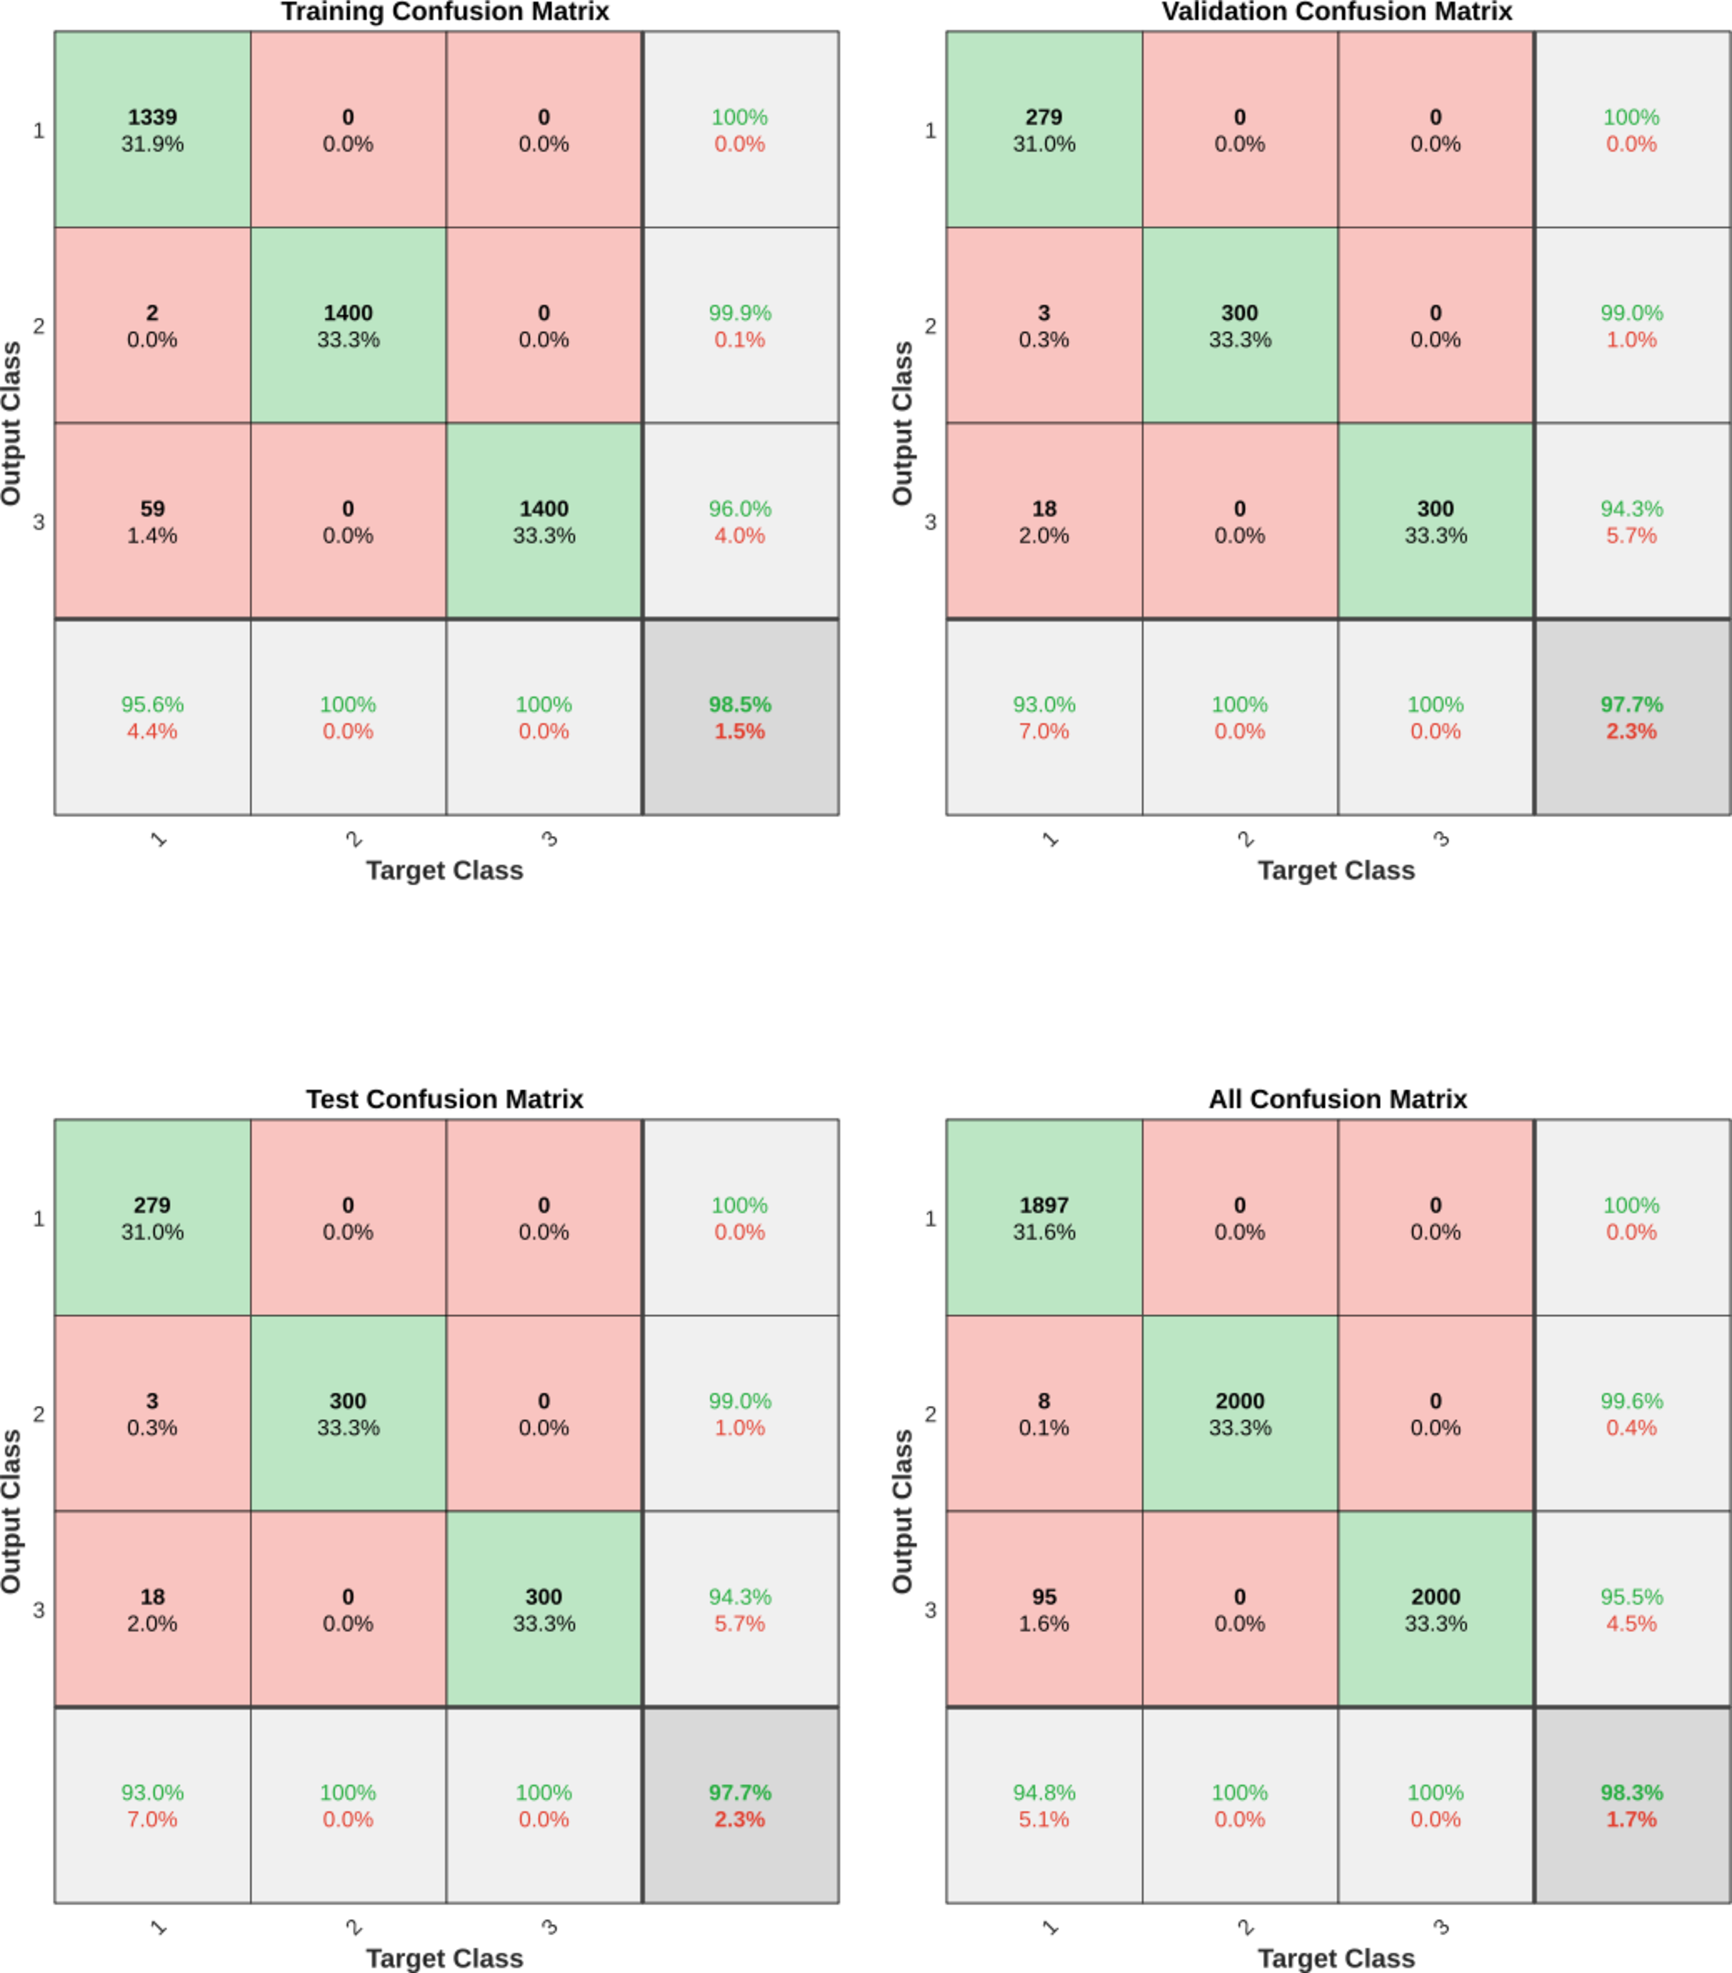
\includegraphics[width=\textwidth]{activityconfusion}
	\caption{Confusion matrices for the activity recognition
	network. Only some samples belonging to the ``sit'' class are
	misclassified.}\label{fig:activityconfusion}
\end{figure}

\begin{figure}[htbp]
	\centering
	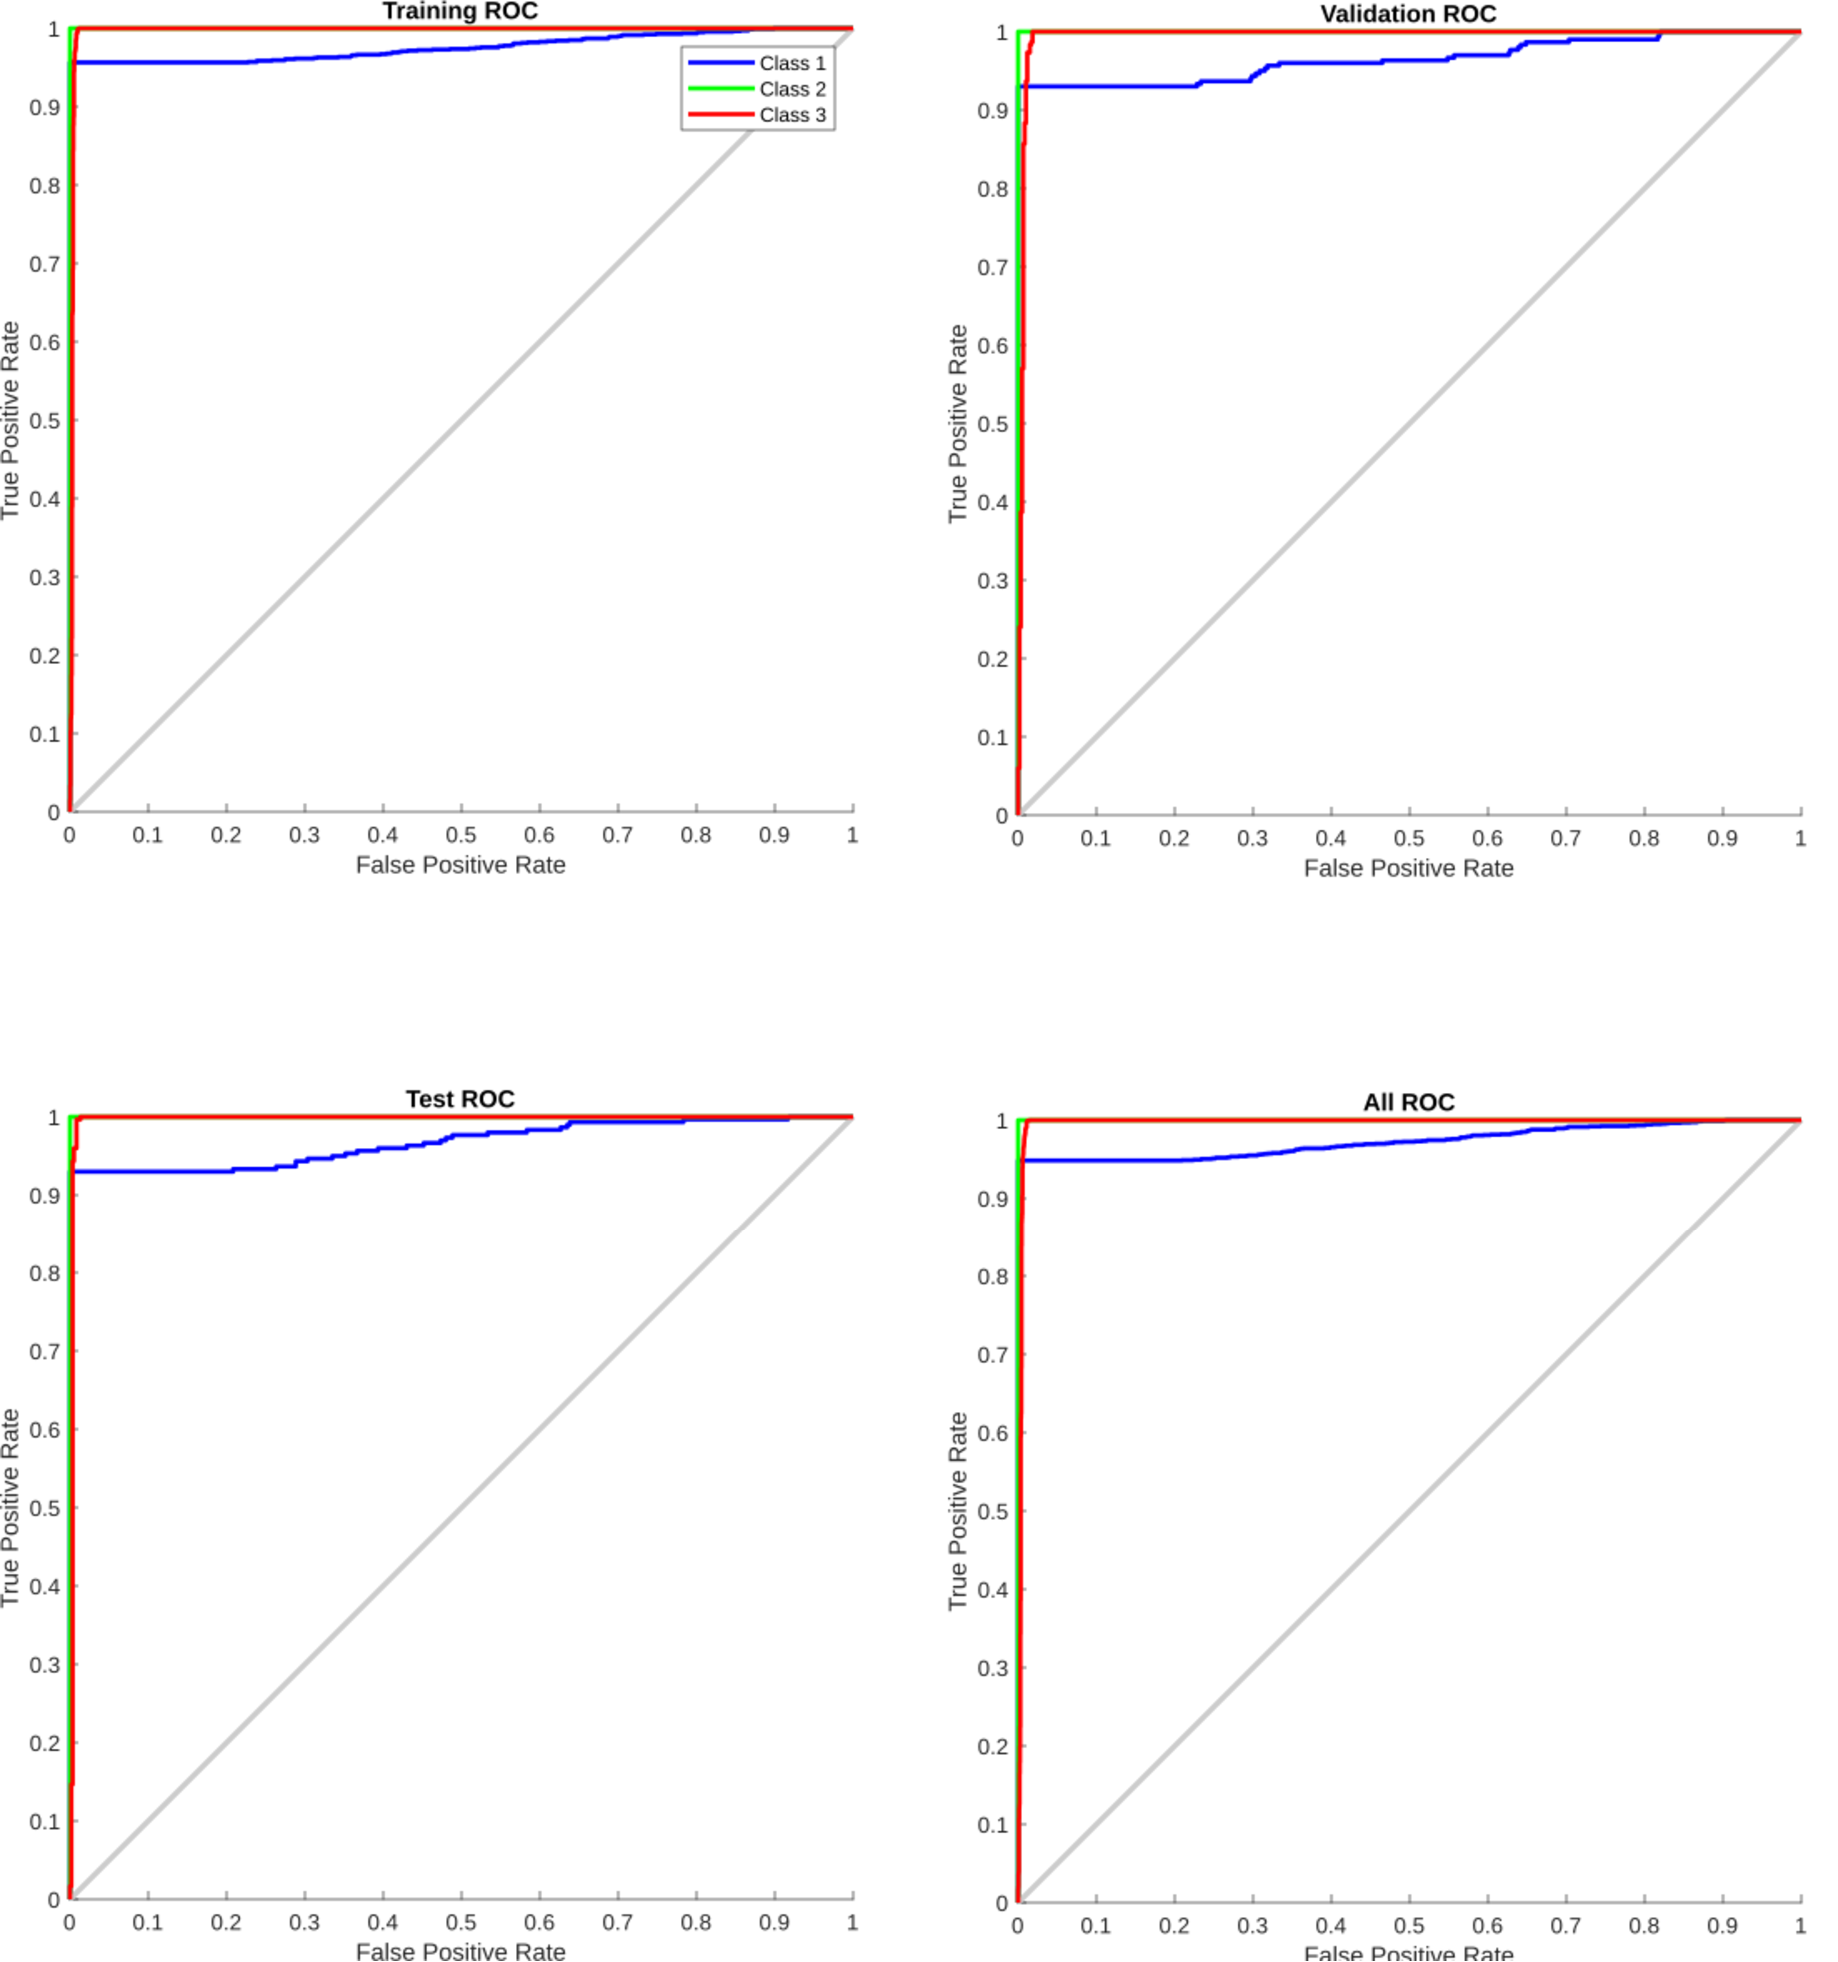
\includegraphics[width=\textwidth]{activityroc}
	\caption{ROC curves for the activity recognition
	network.}\label{fig:activityroc}
\end{figure}
